\documentclass{beamer}
\usepackage{listings}
\lstset{
%language=C,
frame=single, 
breaklines=true,
columns=fullflexible
}
\usepackage{subcaption}
\usepackage{url}

\usepackage{tikz}
\usepackage{pgfplots}
\pgfplotsset{compat=1.17}
\usepackage{tkz-fct}
\usepackage{mathrsfs}
\usepackage{txfonts}
\usepackage{tkz-euclide} 
\usetikzlibrary{calc,math}
\usepackage{float}
\newcommand\norm[1]{\left\lVert#1\right\rVert}
\renewcommand{\vec}[1]{\mathbf{#1}}
\providecommand{\pr}[1]{\ensuremath{\Pr\left(#1\right)}}
\usepackage[export]{adjustbox}
\usepackage[utf8]{inputenc}
\usepackage{amsmath}
\usetheme{Boadilla}
\title{Characteristic Function}
\author{Tanmay Garg - EE20BTECH11048}

\begin{document}
\begin{frame}
\titlepage
\end{frame}
\section{Question}
\begin{frame}{Problem GATE 2015 (MA), Q. 8}
\begin{block}{Question}
Let $X \sim B\left(5,\frac{1}{2}\right)$ and $Y \sim U(0,1)$. The the value of:
\[
    \frac{\pr{X+Y \leq 2}}{\pr{X+Y \geq 5}}
\]
is equal to? ($X$ and $Y$ are independent)

\end{block}
\end{frame}
\begin{frame}{Characteristic function}
   \begin{block}{Definition}
   \begin{enumerate}
       \item It is an alternative way to define the probability mass function or probability density function for a random variable.
       \item It completely defines the probability distribution for the random variable.
   \end{enumerate}
   \end{block}
   \begin{block}{Expression}
   For discrete random variable
   \begin{align}
       C_X(t)= \sum_{k}\pr{X=k}e^{itk}
   \end{align}
   For continuous random variable
   \begin{align}
       C_X(t)=\int_{-\infty}^\infty f_X(x)e^{itx}dx
   \end{align}
   \end{block}
\end{frame}
\begin{frame}{Characteristic function}
\begin{block}{Properties}
\begin{enumerate}
\item It exists for all real value random variables
    \item It is continuous over entire space
    \item It is bounded $|C_X(t)| \leq 1$
    \item If $X$ and $Y$ are independent then 
    \begin{align}
    Z &= X+Y\\
    C_Z(t) &= C_X(t)C_Y(t)
    \end{align}
    \item Gil Pelaez Formula:
    \begin{align}
        \pr{X \leq x}=F_X(x)=\frac{1}{2}-\frac{1}{\pi}\int_0^\infty \frac{\text{Im}\left(e^{-itx}C_X(t)\right)}{t}dt
    \end{align}
\end{enumerate}
\end{block}
\end{frame}
\section{Solution}
\begin{frame}{Solution}
    \begin{block}{Characteristic function of $X$ }
    For $X \sim B\left(5,\frac{1}{2}\right)$ will be(binomial distribution):
\begin{align}
C_X(t) &= \sum_{k}\pr{X=k}e^{itk}\\
&= \sum_{k}{5 \choose k}{\left(\frac{1}{2}\right)}^5e^{itk}\\
   &=\left(\frac{e^{it}+1}{2}\right)^5
\end{align}
    \end{block}
\end{frame}
\begin{frame}{Solution}
    \begin{block}{Characteristic function of $Y$ }
    For $Y \sim U(0,1)$ will be:
\begin{align}
C_Y(t) &= \int_{-\infty}^\infty f_Y(y)e^{ity}dy\\
&= \int_{0}^1\frac{1}{1-0}e^{ity}dy\\
    C_Y(t)&=\frac{e^{it}-1}{it}
\end{align}
    \end{block}
\end{frame}
\begin{frame}{Solution}
\begin{block}{Characteristic function for $Z$}
Since both $X$ and $Y$ are independent we can take:
\begin{align}
    Z&=X+Y\\
    C_Z(t)&=C_X(t)C_Y(t)\\
    C_Z(t)&= \frac{(e^{it}+1)^5(e^{it}-1)}{32it}
\end{align}
Applying Gil-Pelaez formula:
\begin{align}
    F_Z(z)=\frac{1}{2}-\frac{1}{\pi}\int_0^\infty \frac{\text{Im}\left(e^{-itz}C_Z(t)\right)}{t}dt
\end{align}
\begin{align}
    F_Z(z)=\frac{1}{2}-\int_0^\infty\frac{1}{2i\pi t}\left(\frac{(e^{it}+1)^5(e^{it}-1)e^{-itz}+(e^{-it}+1)^5(e^{-it}-1)e^{itz}}{32it}\right)
\end{align}
\end{block}
\end{frame}
\begin{frame}{Solution}
    \begin{block}{$\pr{X+Y \leq 2}$ or $\pr{Z\leq 2}$}
    Substituting $z=2$, the value for $\pr{Z\leq 2}$:
\begin{align}
\nonumber
    &=\frac{1}{2}+\frac{1}{\pi}\int_0^\infty \frac{8\cos{2t}+2\cos{4t}}{64t^2}dt\\
    &\quad+\frac{1}{\pi}\int_0^\infty\frac{+8\cos{3t}-8\cos{t}-10}{64t^2}dt\label{first_sub}
\end{align}
    \end{block}
\end{frame}
\begin{frame}{Solution}
\begin{block}{Integration Method}
Finding a general expression for integrating:
\begin{align}
    \int \frac{\cos{ax}}{x^2}dx=-\frac{\cos{ax}}{x}-a\int\frac{\sin{ax}}{x}dx + C\label{gen1}
\end{align}
By applying integration by parts. Now finding the value of other integral, by substituting $u=ax$ for limits as $0$ and $\infty$:
\begin{align}
    \int_0^\infty\frac{a\sin{ax}}{x}dx &= \int_0^\infty\frac{a\sin{u}}{u}du\\
    &=\frac{a\pi}{2}\label{gen2}
\end{align}
\end{block}
\end{frame}

\begin{frame}{Solution}
    \begin{block}{$\pr{X+Y \leq 2}$ or $\pr{Z\leq 2}$}
    Now using the above general expressions to calculate \eqref{first_sub} and simplifying the expression after putting the limits we get
\begin{align}
\nonumber
    &=\frac{-1}{8\pi}\left(\int_0^\infty\frac{\sin{4t}+3\sin{3t}+2\sin{2t}-\sin{t}}{t}dt\right)\\
    &\quad -\frac{2(\cos{t}-1)(\cos{t}+1)^3}{8\pi t}\bigg|_0^\infty+\frac{1}{2}\\
    &=\frac{1}{2} + \frac{-1}{8\pi}\times \frac{5\pi}{2}+0\\
    &=\frac{3}{16}\label{first_value}
\end{align}
    \end{block}
\end{frame}
\begin{frame}{Solution}
    \begin{block}{$\pr{X+Y\geq 5}$ or $\pr{Z\geq 5}$}
    Similarly on substituting $z=5$, the value for $\pr{Z\leq 5}$:
\begin{align}
\nonumber
    &=\frac{1}{2} +\frac{1}{\pi}\int_0^\infty\frac{-10\cos{3t}-8\cos{4t}}{64t^2}dt\\&\quad +\frac{1}{\pi}\int_0^\infty\frac{-2\cos{5t}+12\cos{t}+8}{64t^2}dt\\ \nonumber
    &=\frac{1}{\pi}\left(\int_0^\infty\frac{5\sin{5t}+16\sin{4t}+15\sin{3t}-6\sin{t}}{32}dt\right)\\
    &\quad+\frac{1}{2}+\frac{1}{\pi}\left(\frac{16(\cos{t}-1)(\cos{t})(\cos{t}+1)^3}{32t}\bigg|_0^\infty\right)\\
    &=\frac{1}{2}+\frac{1}{\pi}\times\frac{15\pi}{32} + 0\\
    &=\frac{31}{32}
\end{align}
    \end{block}
\end{frame}
\begin{frame}{Solution}
\begin{block}{$\pr{X+Y\geq 5}$ or $\pr{Z\geq 5}$}
The value for $\pr{Z\geq 5}$:
\begin{align}
    \pr{Z>5}&=1-\pr{Z\leq 5}\\
    &=1-\frac{31}{32}=\frac{1}{32}\label{second_value}
\end{align}
\end{block}
\end{frame}
\begin{frame}{Solution}
\begin{block}{Final Answer}
Upon substituting \eqref{first_value}and \eqref{second_value}, we get:
\begin{align}
    \frac{\pr{X+Y \leq 2}}{\pr{X+Y \geq 5}} = 6
\end{align}
\begin{figure}[h]
    \centering
    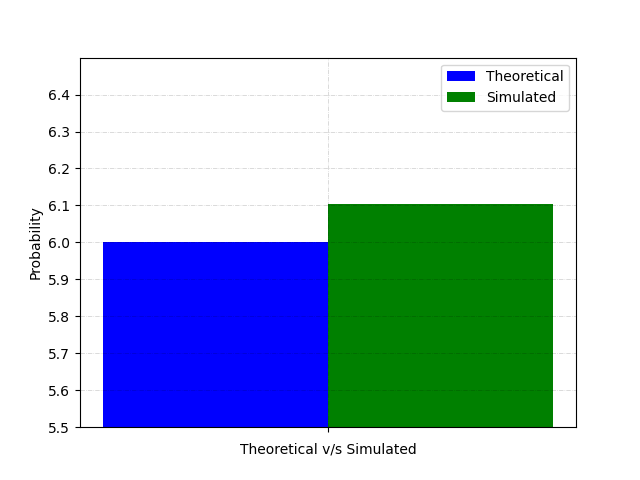
\includegraphics[width =0.5\columnwidth]{Figure_1.png}
    \caption{}
    \label{fig:my_label}
\end{figure}
\end{block}
    
\end{frame}
\end{document}